%%%%%%%%%%%%%%%%%%%%%%%%%%%%%%%%%%%%%%%%%%%%%%%%%%%%%%%%%%%%%

\mainmatter
\setcounter{page}{1}

\lectureseries[\course]{\course}

\auth[\lecAuth]{Lecturer: \lecAuth\\ Scribe: \scribe}
\date{January 5, 2010}

\setaddress

% the following hack starts the lecture numbering at 1
\setcounter{lecture}{0}
\setcounter{chapter}{0}

\lecture{Course Introduction}

\section{Types of Models}
There are several types of models that will be used in this course to describe the behavior of systems including linear and nonlinear models.

\subsection{Linear Time Varying Model}
\begin{align*}
\dot{x} &= A(t)x + B(t)u \\
y &= C(t)x + D(t)u
\end{align*}
Interesting cases of this type arise when there is a high-dimensional state vector and a low-dimensional input vector meaning that a large number of states are trying to be controlled using a small number of inputs or actuators.

\subsection{Nonlinear Model}
\begin{align*}
\dot{x} &= f(t,x,u) \\
y &= h(t,x,u)
\end{align*}

In MAE 281B control design is studied in order to find $u(t,x)$. Note that $u(x)$ is considered a feedback control law while $u(t,x)$ is considered to have a feedforward element as well as feedback. In MAE 281A we will be studying analysis of nonlinear systems without any control or where the control is considered to be an undesirable disturbance to the system.

For terminology Khalil considers $\dot{x}=f(t,x)$ to be a \textit{non-autonomous} system but this can also be thought of as a \textit{time-varying} (TV) system analogous to what is found in the linear control literature. When $\dot{x}=f(x)$ Khalil calls this an \textit{autonomous} system whereas the linear control literature refers to it as \textit{time-invariant} (TI).

\subsection{Time Invariant Systems}
Time invariant systems are described by the relationship
$$\dot{x}=f(x)$$
\begin{definition}
Equilibrium: A point $x=x^\ast$ such that
$$f(x) = 0$$
\end{definition}

\subsection{Linear Time Invariant Systems}
Linear time invariant systems are described by the relationship
$$\dot{x}=Ax$$
\begin{definition}
Equilibria: $\text{null}(A)$ or $\text{kernel}(A)$.
\end{definition}

\section{Multiple Isolated Equilibria}
In the linear case $\dot{x}=Ax$ we have $\text{null}(A)$ is the equilibria manifold or the coninuum of equilibria. In the nonlinear case $\dot{x}=f(x)$ we find multiple isolated equilibria.
\begin{example}
Let
$$\dot{x} = x-x^3 = x(1-x^2)$$
The equilibria are found when $f(x)=0$ which in this case leads to $x=0,\pm1$. Figure \ref{fig:01roots} shows where the equilibria lie on a line and Figure \ref{fig:01traj} shows how the solution depends on the initial conditions. The highlighted initial conditions are when $x_0\gg1$, $x_0\ll1$, $0<x_0<1$ and $-1<x_0<0$. Later in this course we will see that the $\pm1$ equilibria are attracting and the $0$ equilibria is repellant and that attracting equilibria are stable while repellant equilibria are unstable.
$\lozenge$
\end{example}

\begin{figure}[ht!]
	\centering
	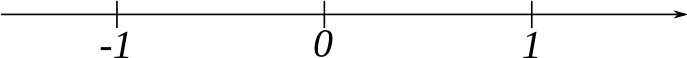
\includegraphics[width=.4\textwidth]{images/01roots}
	\caption{Equilibria points.}
	\label{fig:01roots}
\end{figure}

\begin{figure}[ht!]
	\centering
	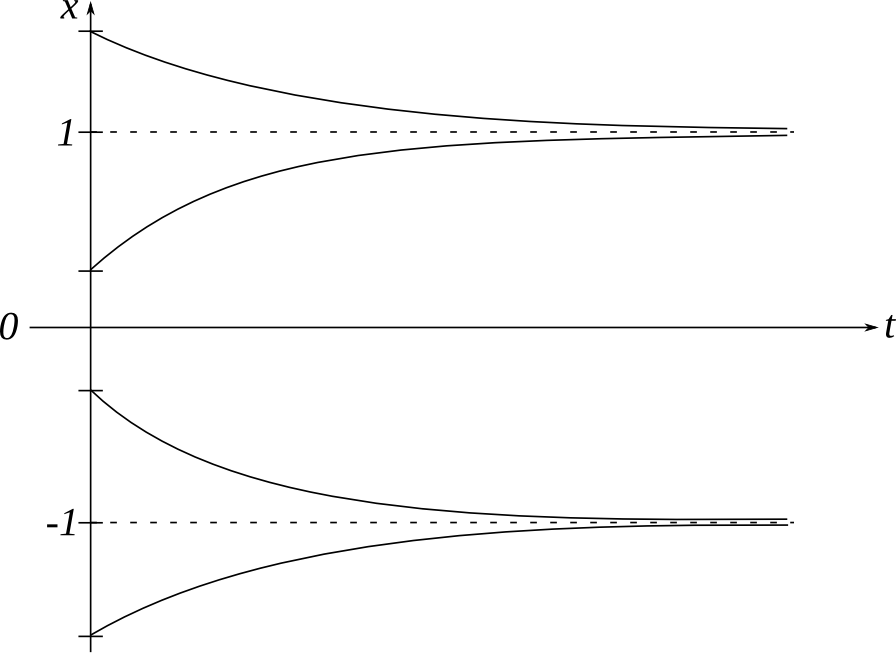
\includegraphics[width=.4\textwidth]{images/01traj}
	\caption{State trajectory.}
	\label{fig:01traj}
\end{figure}

\section{Finite Escape Time}
\begin{example}
A linear unstable system is given by
$$\dot{x} = x \Rightarrow x(t) = x_0e^t$$
$\lozenge$
\end{example}

\begin{example}
A nonlinear unstable system is given by
$$\dot{x} = x^3 \Rightarrow \frac{dx}{dt}=x^3 \Rightarrow \int\frac{dx}{x^3} = \int dt \Rightarrow x(t) = \frac{x_0}{\sqrt{1-2x_0^2t}}$$
This solution blows up as $t\to\frac{1}{2x_0^2}$ because then there is a division by zero, see Figure \ref{fig:01blowup}. Notice that for smaller initial conditions the system blows up later than for larger initial conditions. The rule of thumb is to pay special attention to instabilities larger than linear in growth.
$\lozenge$
\end{example}

\begin{figure}[ht!]
	\centering
	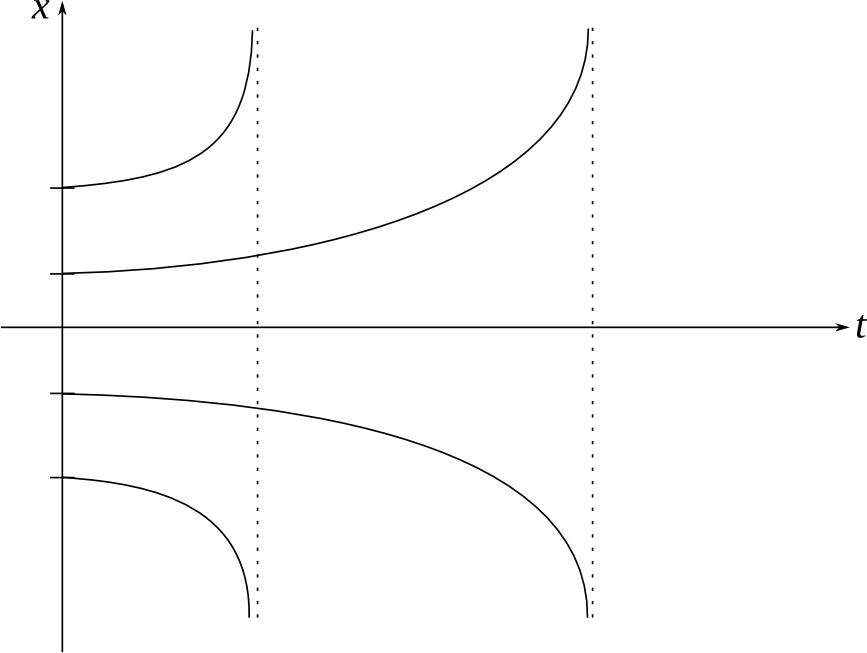
\includegraphics[width=.4\textwidth]{images/01blowup}
	\caption{Effect of initial conditions on stability.}
	\label{fig:01blowup}
\end{figure}

\section{Limit Cycle}
\begin{example}
A linear limit cycle is given by a second order linear harmonic system such as an LC circuit or a mass-spring system where
$$\ddot{x} + x = 0$$
See Figure \ref{fig:01secondorder}.
$\lozenge$
\end{example}

\begin{figure}[ht!]
	\centering
	\includegraphics[width=.4\textwidth]{images/01secondorder}
	\caption{Oscillation for a second order linear system.}
	\label{fig:01secondorder}
\end{figure}

\begin{example}
A nonlinear limit cycle is given by a Van der Pol oscillator where
$$\ddot{x} + (x^2-1)\dot{x} + x = 0$$
Here the position term and the viscosity term tend to balance each other out so that as one increases the other decreases and vice-versa.
$\lozenge$
\end{example}
%%%%%%%%%%%%%%%%%%%%%%%%%%%%%%%%%%%%%%%%%%%%%%%%%%%%%%%%%%%%%